\chapter{Обзор предметной области}
Оптическое волокно — нить из оптически прозрачного материала (стекло, пластик), используемая для переноса света внутри себя посредством полного внутреннего отражения. Для объяснения этого явления рассмотрим процессы происходящие при прохождении светом границы двух сред:

При переходе из одной среды в другую с отличающимся показателем преломления свет отклоняется от направления своего распространения. Величина этого отклонения определяется законом Снеллиуса:

\begin{equation}
 n_1 \sin\theta_1 = n_2 \sin\theta_2
\end{equation}

\begin{figure}[h!]
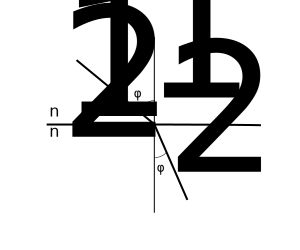
\includegraphics[width=0.5\textwidth]{img/refraction.pdf}
\caption{Преломление света}
\end{figure}

Очевидно, что при некотором угле падения синус соответствующего угла преломления окажется больше единицы, что невозможно. В этом случае будет наблюдаться эффект полного внутреннего отражения (ПВО). Это возможно только в случае $n_1 > n_2$

\begin{figure}[h!]
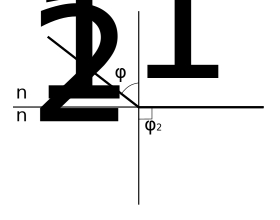
\includegraphics[width=0.5\textwidth]{img/refraction_full_inner.pdf}
\caption{Полное внутреннее отражение}
\end{figure}

\section{Классификация световодов}
Волновод — это структура, способная поддерживать распространяющиеся вдоль него волны, поля которых сосредоточены внутри волновода или в примыкающей к нему области. По строению оптические световоды делятся на несколько типов:

\begin{figure}[h!]
	\begin{minipage}[h]{0.32\linewidth}
		\center{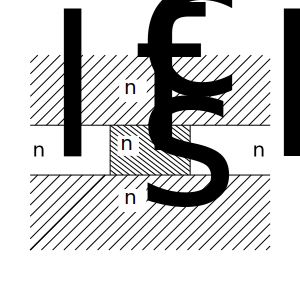
\includegraphics[width=1\linewidth]{img/polozok_a.pdf} \\ а)}
	\end{minipage}
	\hfill
	\begin{minipage}[h]{0.32\linewidth}
		\center{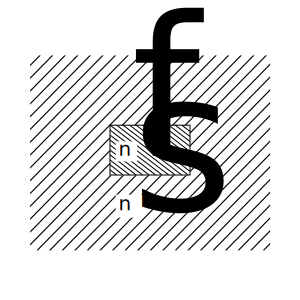
\includegraphics[width=1\linewidth]{img/polozok_b.pdf} \\ б)}
	\end{minipage}
	\hfill
	\begin{minipage}[h]{0.32\linewidth}
		\center{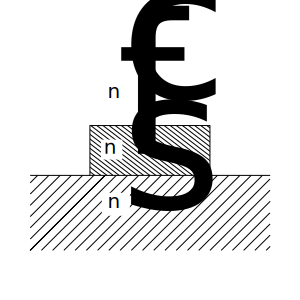
\includegraphics[width=1\linewidth]{img/polozok_c.pdf} \\ в)}
	\end{minipage}
	\vfill
	\begin{minipage}[h]{0.32\linewidth}
		\center{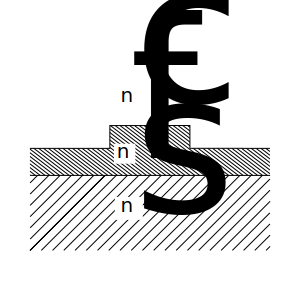
\includegraphics[width=1\linewidth]{img/polozok_d.pdf} \\ г)}
	\end{minipage}
	\hfill
	\begin{minipage}[h]{0.32\linewidth}
		\center{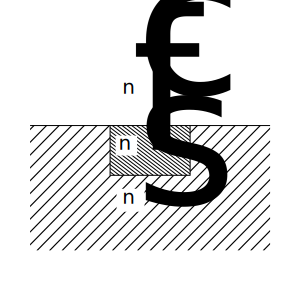
\includegraphics[width=1\linewidth]{img/polozok_e.pdf} \\ д)}
	\end{minipage}
	\hfill
	\begin{minipage}[h]{0.32\linewidth}
		\center{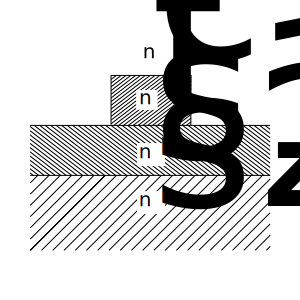
\includegraphics[width=1\linewidth]{img/polozok_f.pdf} \\ е)}
	\end{minipage}	
	\caption{Типы полосковых волноводов: а)~общий случай, б)~погруженный, в)~приподнятый, г)~гребенчатый, д)~внедренный, е)~составной}
	\label{planars}
\end{figure}

\begin{itemize}
\item Планарный световод - представляет собой полоски прямоугольного сечения (сердцевины), окруженные сверху и снизу слоями диэлектрика с меньшим показателем преломления, чем в сердцевине. Планарный волновод называется симметричным, если показатели преломления сверху и снизу равны, и асимметричным, если нет.
\item Полосковый световод - имеет аналогичную структуру, но его сердцевина ограничена со всех четырех сторон, в отличие от планарного. По способу формирования делится на несколько типов, показанных на рисунке.
\item Оптическое волокно - представляет собой нить, имеющую, как правило, круглое или эллиптическое сечение.
\end{itemize} 

\begin{figure}[h!]
	\begin{minipage}[h]{0.49\linewidth}
		\center{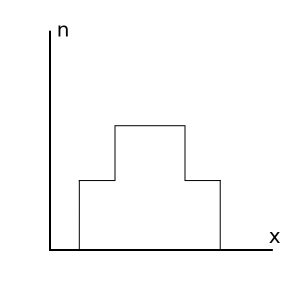
\includegraphics[width=1\linewidth]{img/cylinder_sf.pdf} \\ а)}
	\end{minipage}
	\hfill
	\begin{minipage}[h]{0.49\linewidth}
		\center{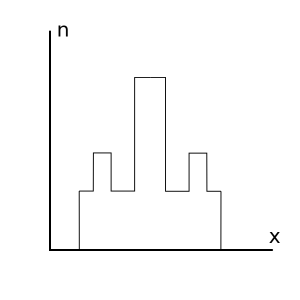
\includegraphics[width=1\linewidth]{img/cylinder_dsf.pdf} \\ б)}
	\end{minipage}
	\caption{Профили показателей преломления цилиндрических волноводов: а)~ступенчатый (SF), б)~специальный (DSF, NZDSF)}
	\label{cylinders}
\end{figure}

Оптические волокна подразделяются на одномодовые и многомодовые, в зависимости от числа распространяющихся в нем мод. В настоящее время в основном используют одномодовые волокна. Распространение только одной моды устраняет межмодовую дисперсию и обеспечивает высокую пропускную  способность одномодового волокна в окнах прозрачности.

Существуют следующие модификации одномодовых волокон:
\begin{itemize}
\item Стандартное  волокно (SF, standart fiber). В этом волокне диаметр светонесущей жилы составляет 8-10 мкм и сравним с длиной световой волны. Одномодовый  режим  реализуется  в  окнах  прозрачности 1310 и 1550 нм. Наилучший  режим  распространения  с точки зрения дисперсии достигается  в  окрестности  длины  волны 1310~нм,  когда  хроматическая  дисперсия обращается в ноль. При этом потери составляют $0,3-0,4$ дБ/км,  в  то  время,  как  наименьшее  затухание $0,2-0,25$ дБ/км достигается в окне 1550 нм. 
\item Волокно со смещенной дисперсией (DSF). Имеет специальный профиль показателя преломления волокна. В итоге длина  волны  нулевой  дисперсии $\lambda_0$ смещена в окно 1550 нм. Таким  образом,  в  волокне  со  смещенной дисперсией реализуются наилучшие характеристики как по минимуму дисперсии, так и по минимуму  потерь.  Поэтому  такое  волокно  лучше  подходит  для  строительства протяженных  высокоскоростных  линий  связи  с  расстоянием  между  переприемными участками до 100 и более км. 
\item Волокно  с  ненулевой  смещенной  дисперсией NZDSF  в  отличие  от DSF 
оптимизировано  для  передачи  не  одной  длины  волны,  а  сразу  нескольких  длин  волн 
(сигнала  со  спектральным  уплотнением WDM). Длина волны нулевой дисперсии у этого волокна, в отличие от волокна DSF, выведена за пределы этого диапазона, что значительно ослабляет влияние нелинейных эффектов в окрестности точки нулевой дисперсии при распространении по волокну нескольких длин волн.
\end{itemize}    

\section{Планарные и полосковые волноводы}

\begin{figure}[h!]
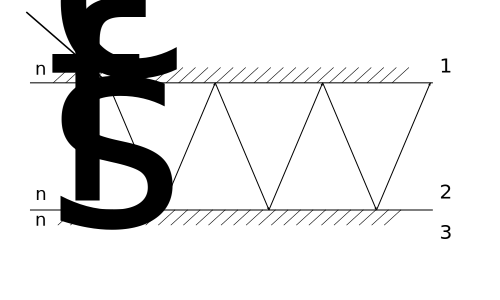
\includegraphics[width=0.9\textwidth]{img/planar_propagation.pdf}
\caption{Распространение света в волноводе}
\end{figure}

Планарный волновод - это структура из как минимум трех слоев с разными показателями преломления с соотношением $n_f > n_s > n_c$ С точки зрения геометрической оптики, свет, попадая в волновод, испытывает ПВО последовательно от обеих границ и оказывается заключен в волноводной среде и распространяется вдоль нее с максимальной эффективностью. Найдем распределение поля электромагнитных волн в волноводе из уравнений Максвелла \cite{adams}:

\begin{equation}
 	\nabla\times \mathbf{H} = -n_j^2\epsilon_0 \frac{d\mathbf{E}}{dt},
 	\label{makswell_1}
\end{equation}
\begin{equation}
	\nabla\times \mathbf{E} = -\mu_0\frac{d\mathbf{H}}{dt},
  	\label{makswell_2}
\end{equation}
\begin{equation}
 	\nabla\cdot \mathbf{E} = 0,
 	\label{makswell_3}
\end{equation}
\begin{equation}
 	\nabla\cdot \mathbf{H} = 0.
 	\label{makswell_4} 
\end{equation}

Подставив в уравнение (\ref{makswell_2}) величину $H$ из уравнения (\ref{makswell_1}) и применив оператор дивергенции, получим:

\begin{equation}
	\nabla^2\mathbf{E} = -\mu_0\epsilon_0 n_j^2 \frac{d^2\mathbf{E}}{dt^2}.
\end{equation}

Предполагая искомое решение в виде $E \sim \exp(-i\omega t)$, получим волновое уравнение:

\begin{equation}
	\nabla^2\mathbf{E} + k^2 n_j^2 E = 0,
\end{equation}

где $k^2 = \omega^2\mu_0 \epsilon_0$. Учитывая, что планарный волновод не ограничен положительном и отрицательном направлениях по оси y, то распределение поля однородно, а производная обращается в нуль. Кроме того, допустим, что по координате z определяется как $\exp(i\beta z)$, где $\beta$ - постоянная распространения, то уравнение для каждой из областей волновода запишется так:

\begin{equation}
	\frac{\partial^2 E_3}{\partial x^2} -(\beta^2 - n_3^2 k^2)E_3 = 0
\end{equation}

\begin{equation}
	\frac{\partial^2 E_1}{\partial x^2} -(n_1^2 k^2 - \beta^2)E_1 = 0
\end{equation}

\begin{equation}
	\frac{\partial^2 E_2}{\partial x^2} -(\beta^2 - n_2^2 k^2)E_2 = 0
\end{equation}

Большая часть энергии моды должна быть сосредоточена в центральной области с показателем преломления $n_1$. Этому условию подойдет решение, осциллирующее в области 1 и затухающее за ее пределами в областях 2 и 3. Поэтому запишем распределение поля в виде:

\begin{equation}
	E_y =
	\begin{cases}
		Ae^{-rx}, &\text{если $x \geqslant 0$;}\\
		A\cos qx + B\sin qx, &\text{если $0 \geqslant x \geqslant -2a $;}\\
		(A\cos 2aq + B\sin 2aq)e^{p(x+2a)}, &\text{если $-2a \geqslant x$.}
	\end{cases}
\end{equation}

Полосковые волноводы отличаются от планарных изменением показателя преломления не только сверху и снизу, но и по бокам. Они используются в качестве направляющих структур оптических устройств и соединительных линий оптических цепей. Достаточно сильное ограничение полей направляемых мод в поперечном сечении позволяет уменьшить их размер и, в конечном счете, размер всех оптической схемы. Более того, прямоугольная форма сечения является простой в изготовлении. Для этого используются метод ионного обмена, диффузии титана в подложку из ниобата лития, протонный обмен или получение волноводных структур на основе матриц из пористого стекла\cite{vlada}. Эти технологии хорошо отработаны и дают волноводы подходящего качества.
Расчет канальных оптических волноводов сложнее чем для планарных, поскольку добавляются еще две плоскости раздела двух сред. Существует несколько видов расчета, такие как метод метод Гоелля; метод Шлессера-Унгера; универсальный метод Маркатили; решение характеристического уравнения в нормированных переменных или через переменные u, v, w; метод эффективного показателя преломления и другие.

\section{Цилиндрические волноводы}
\label{cylinder_waveguides}
Наряду с волноводами прямоугольного сечения применяются также цилиндрические волноводы круглого сечения. Как правило, такие волноводы состоят из сердцевины с высоким показателем преломления и оболочки с меньшим показателем преломления. 

\begin{figure}[h!]
	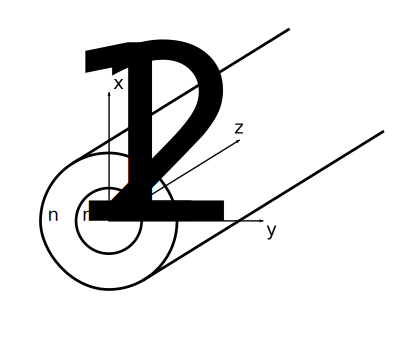
\includegraphics[width=0.7\textwidth]{img/cylinder_axes.pdf}
	\caption{Цилиндрический волновод}
\end{figure}

Для нахождения распределения поля воспользуемся волновым уравнением в цилиндрических координатах:

\begin{equation}
	\frac{\partial^2\psi}{\partial r^2} + \frac{1}{r}\frac{\partial\psi}{\partial r}+\frac{1}{r^2}\frac{\partial^2\psi}{\partial\theta^2}+(n_j^2 k^2 - \beta^2)\psi = 0.
\end{equation}

Так как мы ищем решение с круговой симметрией, то общее решение будет иметь вид:

\begin{equation}
	\psi(r, \theta) = R(r)e^{i\nu\theta} \qquad (\nu = 0,1,2, ...),
\end{equation}

Где $\psi(r, \theta)$ - это продольная составляющая поля, $E_z$ или $H_z$. Подставляя решение в уравнение, получим:

\begin{equation}
	\frac{\partial^2 R}{\partial r^2} + \frac{1}{r}\frac{\partial R}{\partial r}+(n_j^2 k^2 - \beta^2 - \frac{\nu^2}{r^2}) = 0.
\end{equation}

Здесь возможны два варианта решения, для TE-мод, когда $E_z = 0$ и TM ($H_z = 0$). Найдем решение для TE-моды, в случае TM, уравнение решается аналогично

\begin{equation}
	H_z = H_0 J_v (\frac{ur}{a}),
	\label{cylinder_bessel}
\end{equation}

где $J_v$ - функция Бесселя, $v = 0, 1, 2,\ldots$, $\frac{u}{a} = \sqrt{k^2 n_j^2 - \beta^2}$. В зависимости от параметра $v$ мы получим распределение поля различных мод. Интегрально-оптические схемы, в основном, функционируют в одномодовом режиме поскольку в нем отсутствует межмодовая дисперсия и получается меньше помех.